\renewcommand{\chaptername}{Appendix}
\setcounter{chapter}{0}
\renewcommand{\thechapter}{\Alph{chapter}}

\chapter{Plots}

This appendix contains all of the plots that weren't significant enough to include in chapters \ref{chap:toy-dataset} and \ref{chap:cisco-dataset}.

\begin{figure}
  \centering
  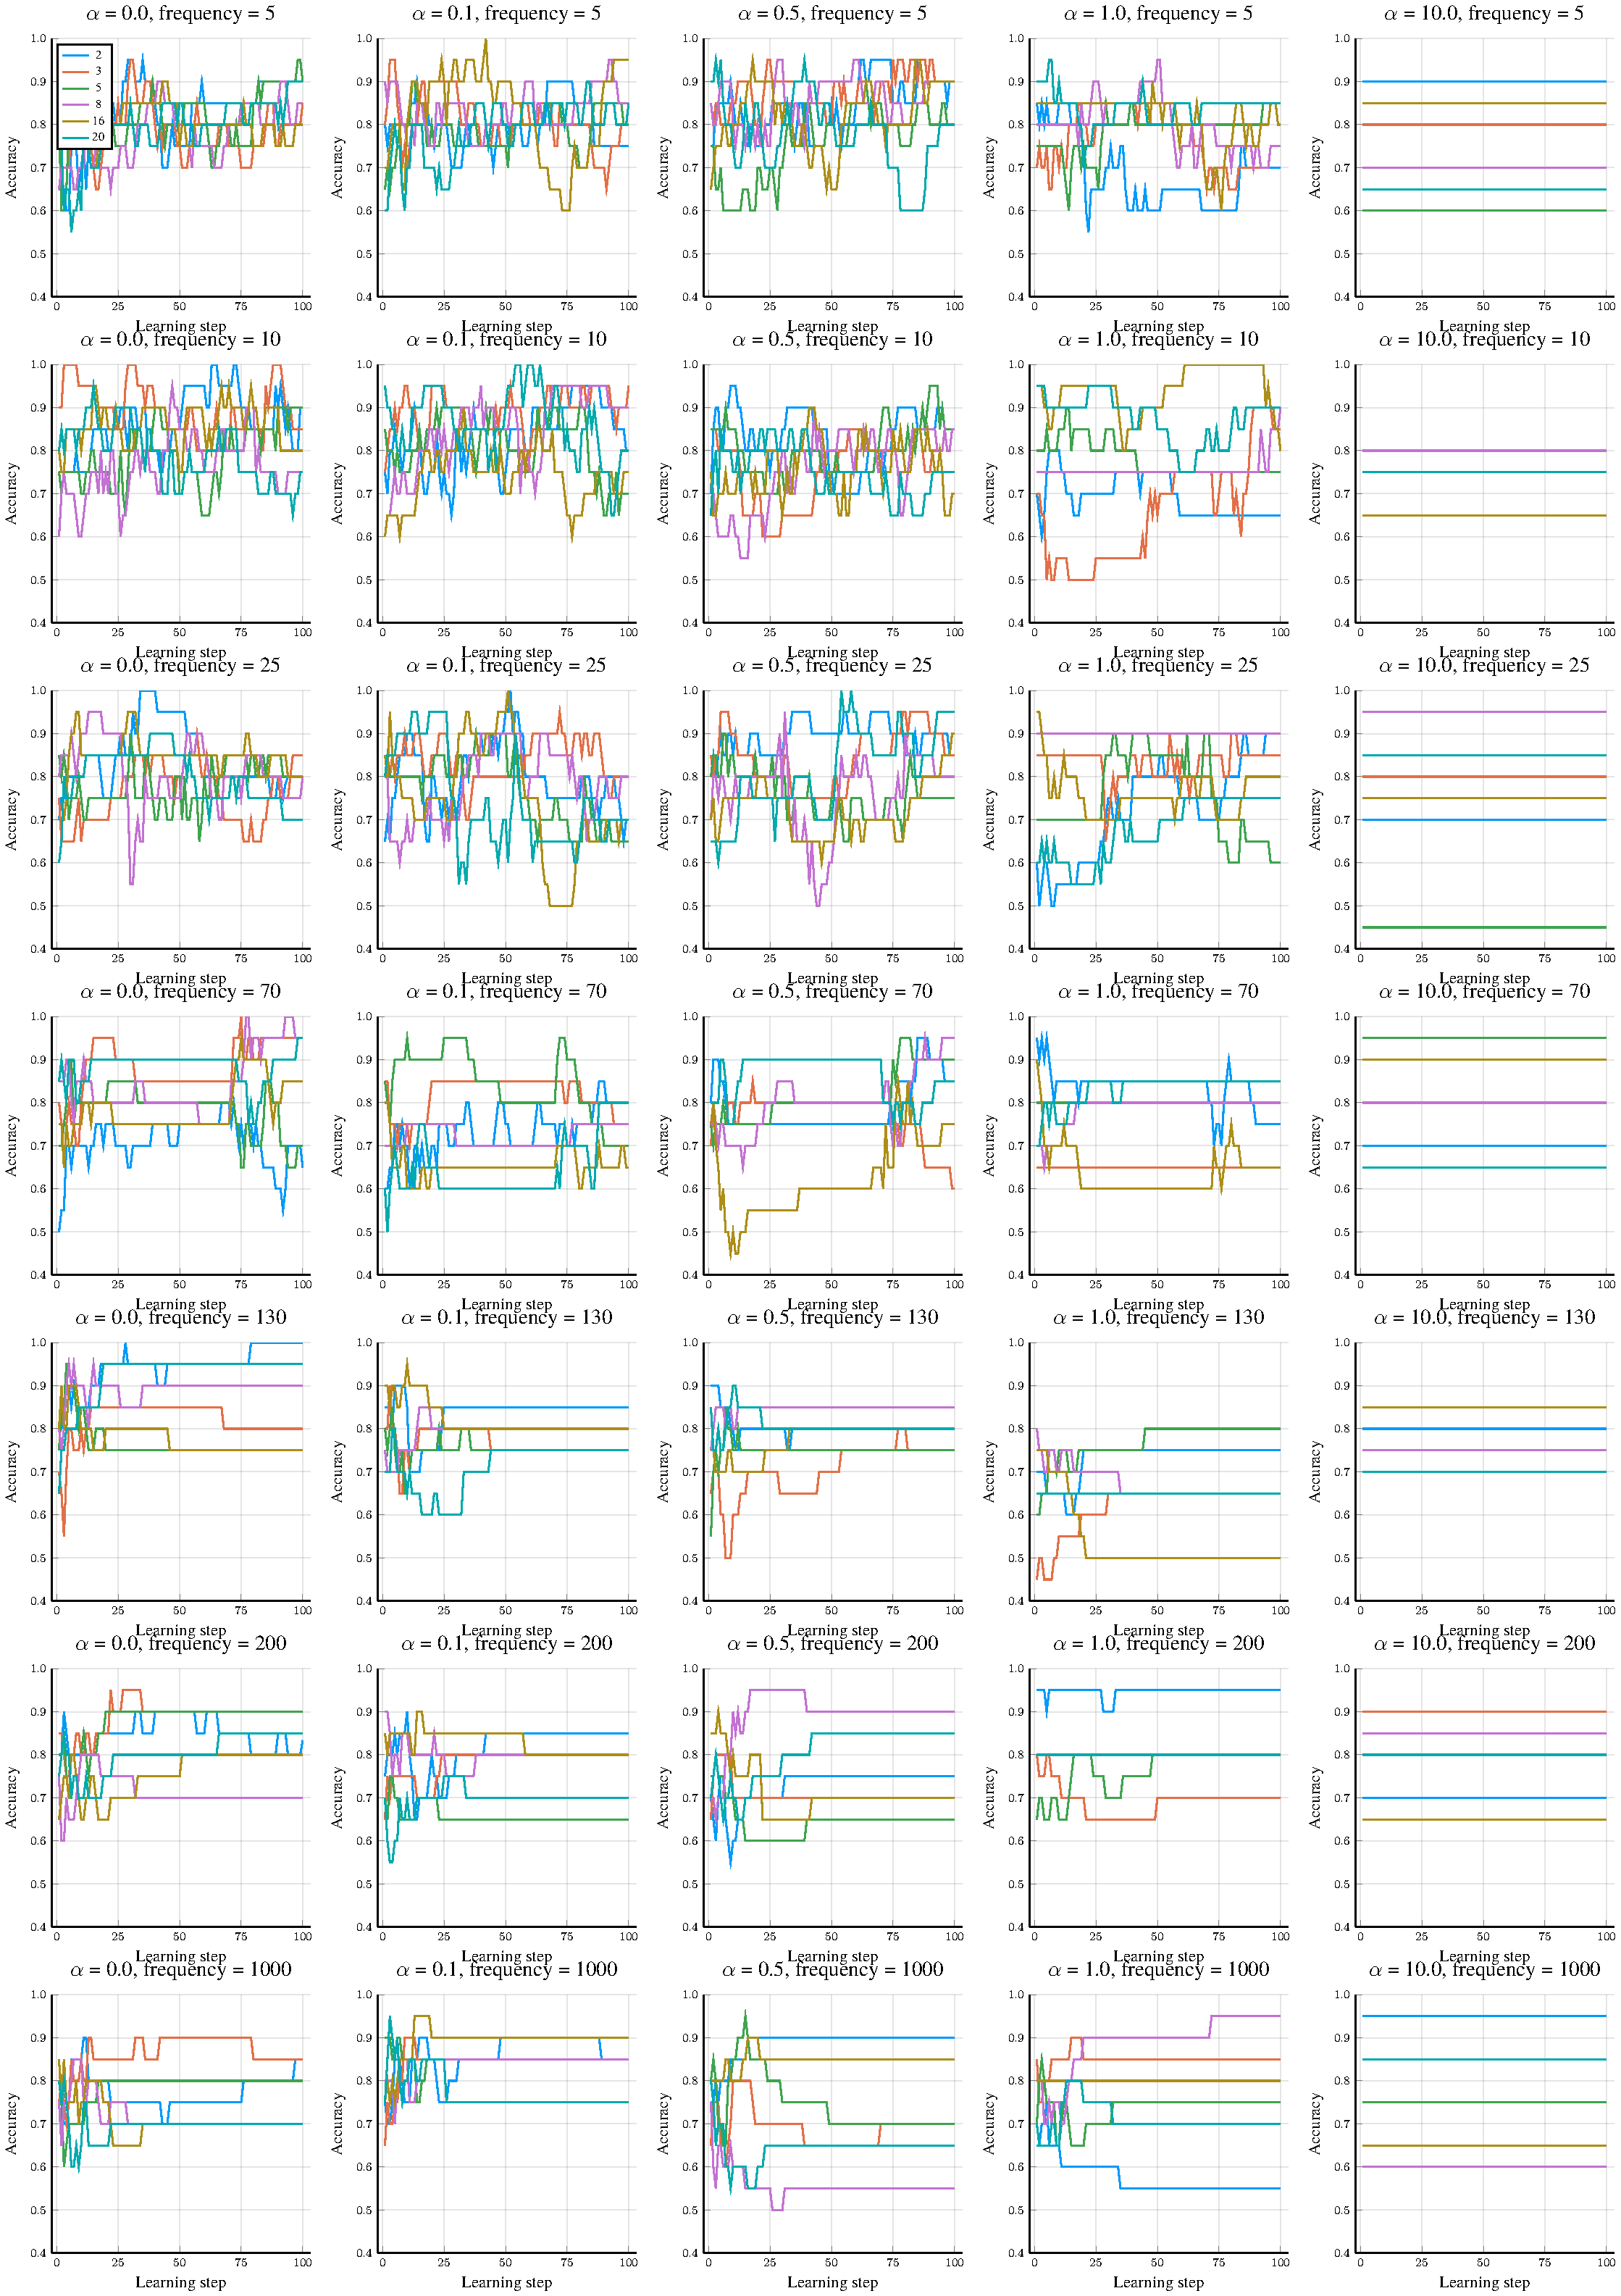
\includegraphics[width=0.93\textwidth]{images/magnet-gridsearch/accuracy/K/magnet-gridsearch-accuracy-K.pdf}
  \caption{The accuracy of a kNN classifier built on the embedding over the learning period for different values of \( K \), \( \alpha \) and the cluster index update frequency for magnet loss. Each subplot corresponds to a particular \( \alpha \) and the cluster index update frequency. The series in each subplot correspond to a value of \( K \).}\label{fig:magnet-gridsearch-accuracy}
\end{figure}

\begin{figure}
  \centering
  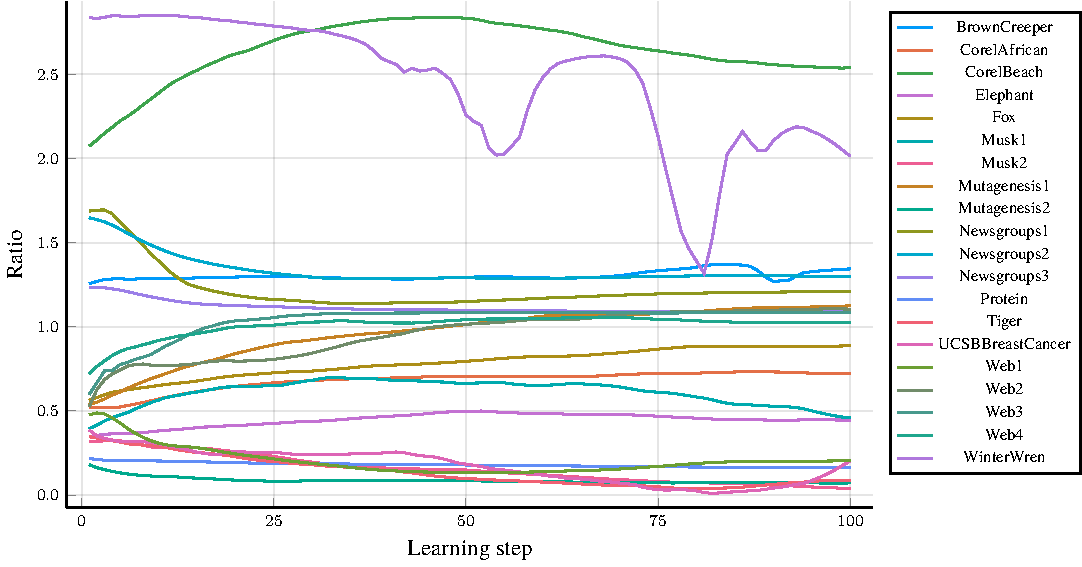
\includegraphics[width=\textwidth]{images/CPC-toy/ratio/CPC-toy-ratio.pdf}
  \caption{The value of \( \mathrm{silhouette} \left( \cdot \right) \) for \( L_\mathrm{CPC} \) over the learning period.}\label{fig:CPC-toy-ratio}
\end{figure}

\begin{figure}
  \centering
  \begin{subfigure}[t]{\textwidth}
    \centering
    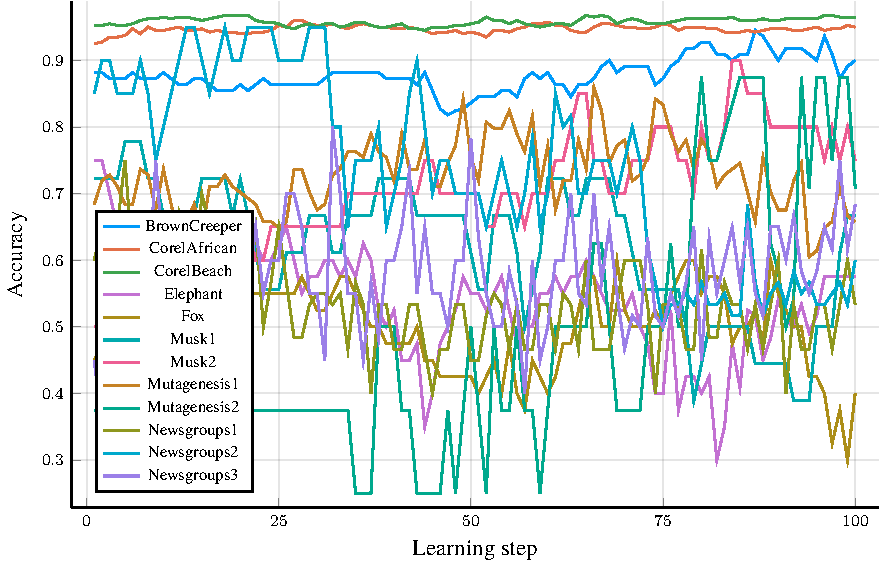
\includegraphics[width=\textwidth]{images/CPC-toy/accuracy1/CPC-toy-accuracy1.pdf}
  \end{subfigure}
  \begin{subfigure}[t]{\textwidth}
    \centering
    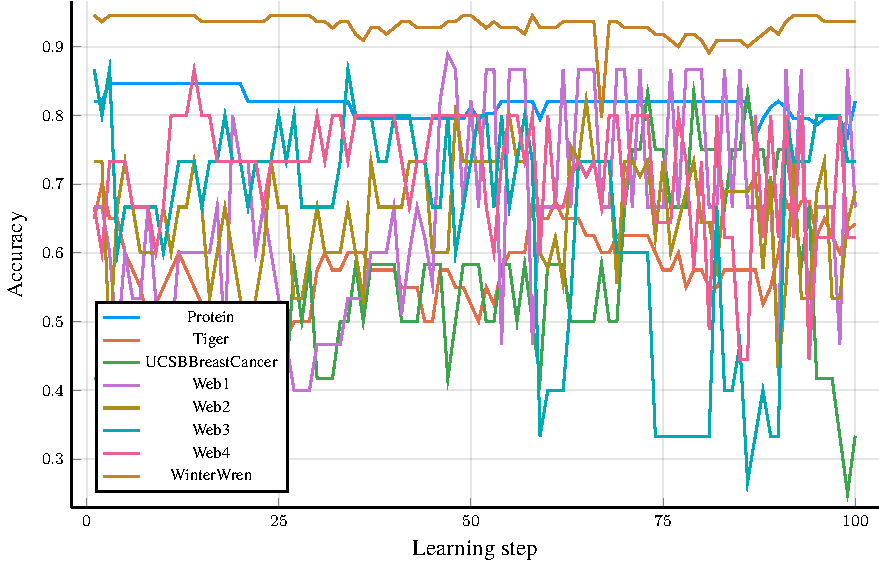
\includegraphics[width=\textwidth]{images/CPC-toy/accuracy2/CPC-toy-accuracy2.pdf}
  \end{subfigure}
  \caption{The accuracy of a kNN classifier built on the embedding for \( L_\mathrm{CPC} \) over the learning period.}\label{fig:CPC-toy-accuracy}
\end{figure}

\begin{figure}
  \centering
  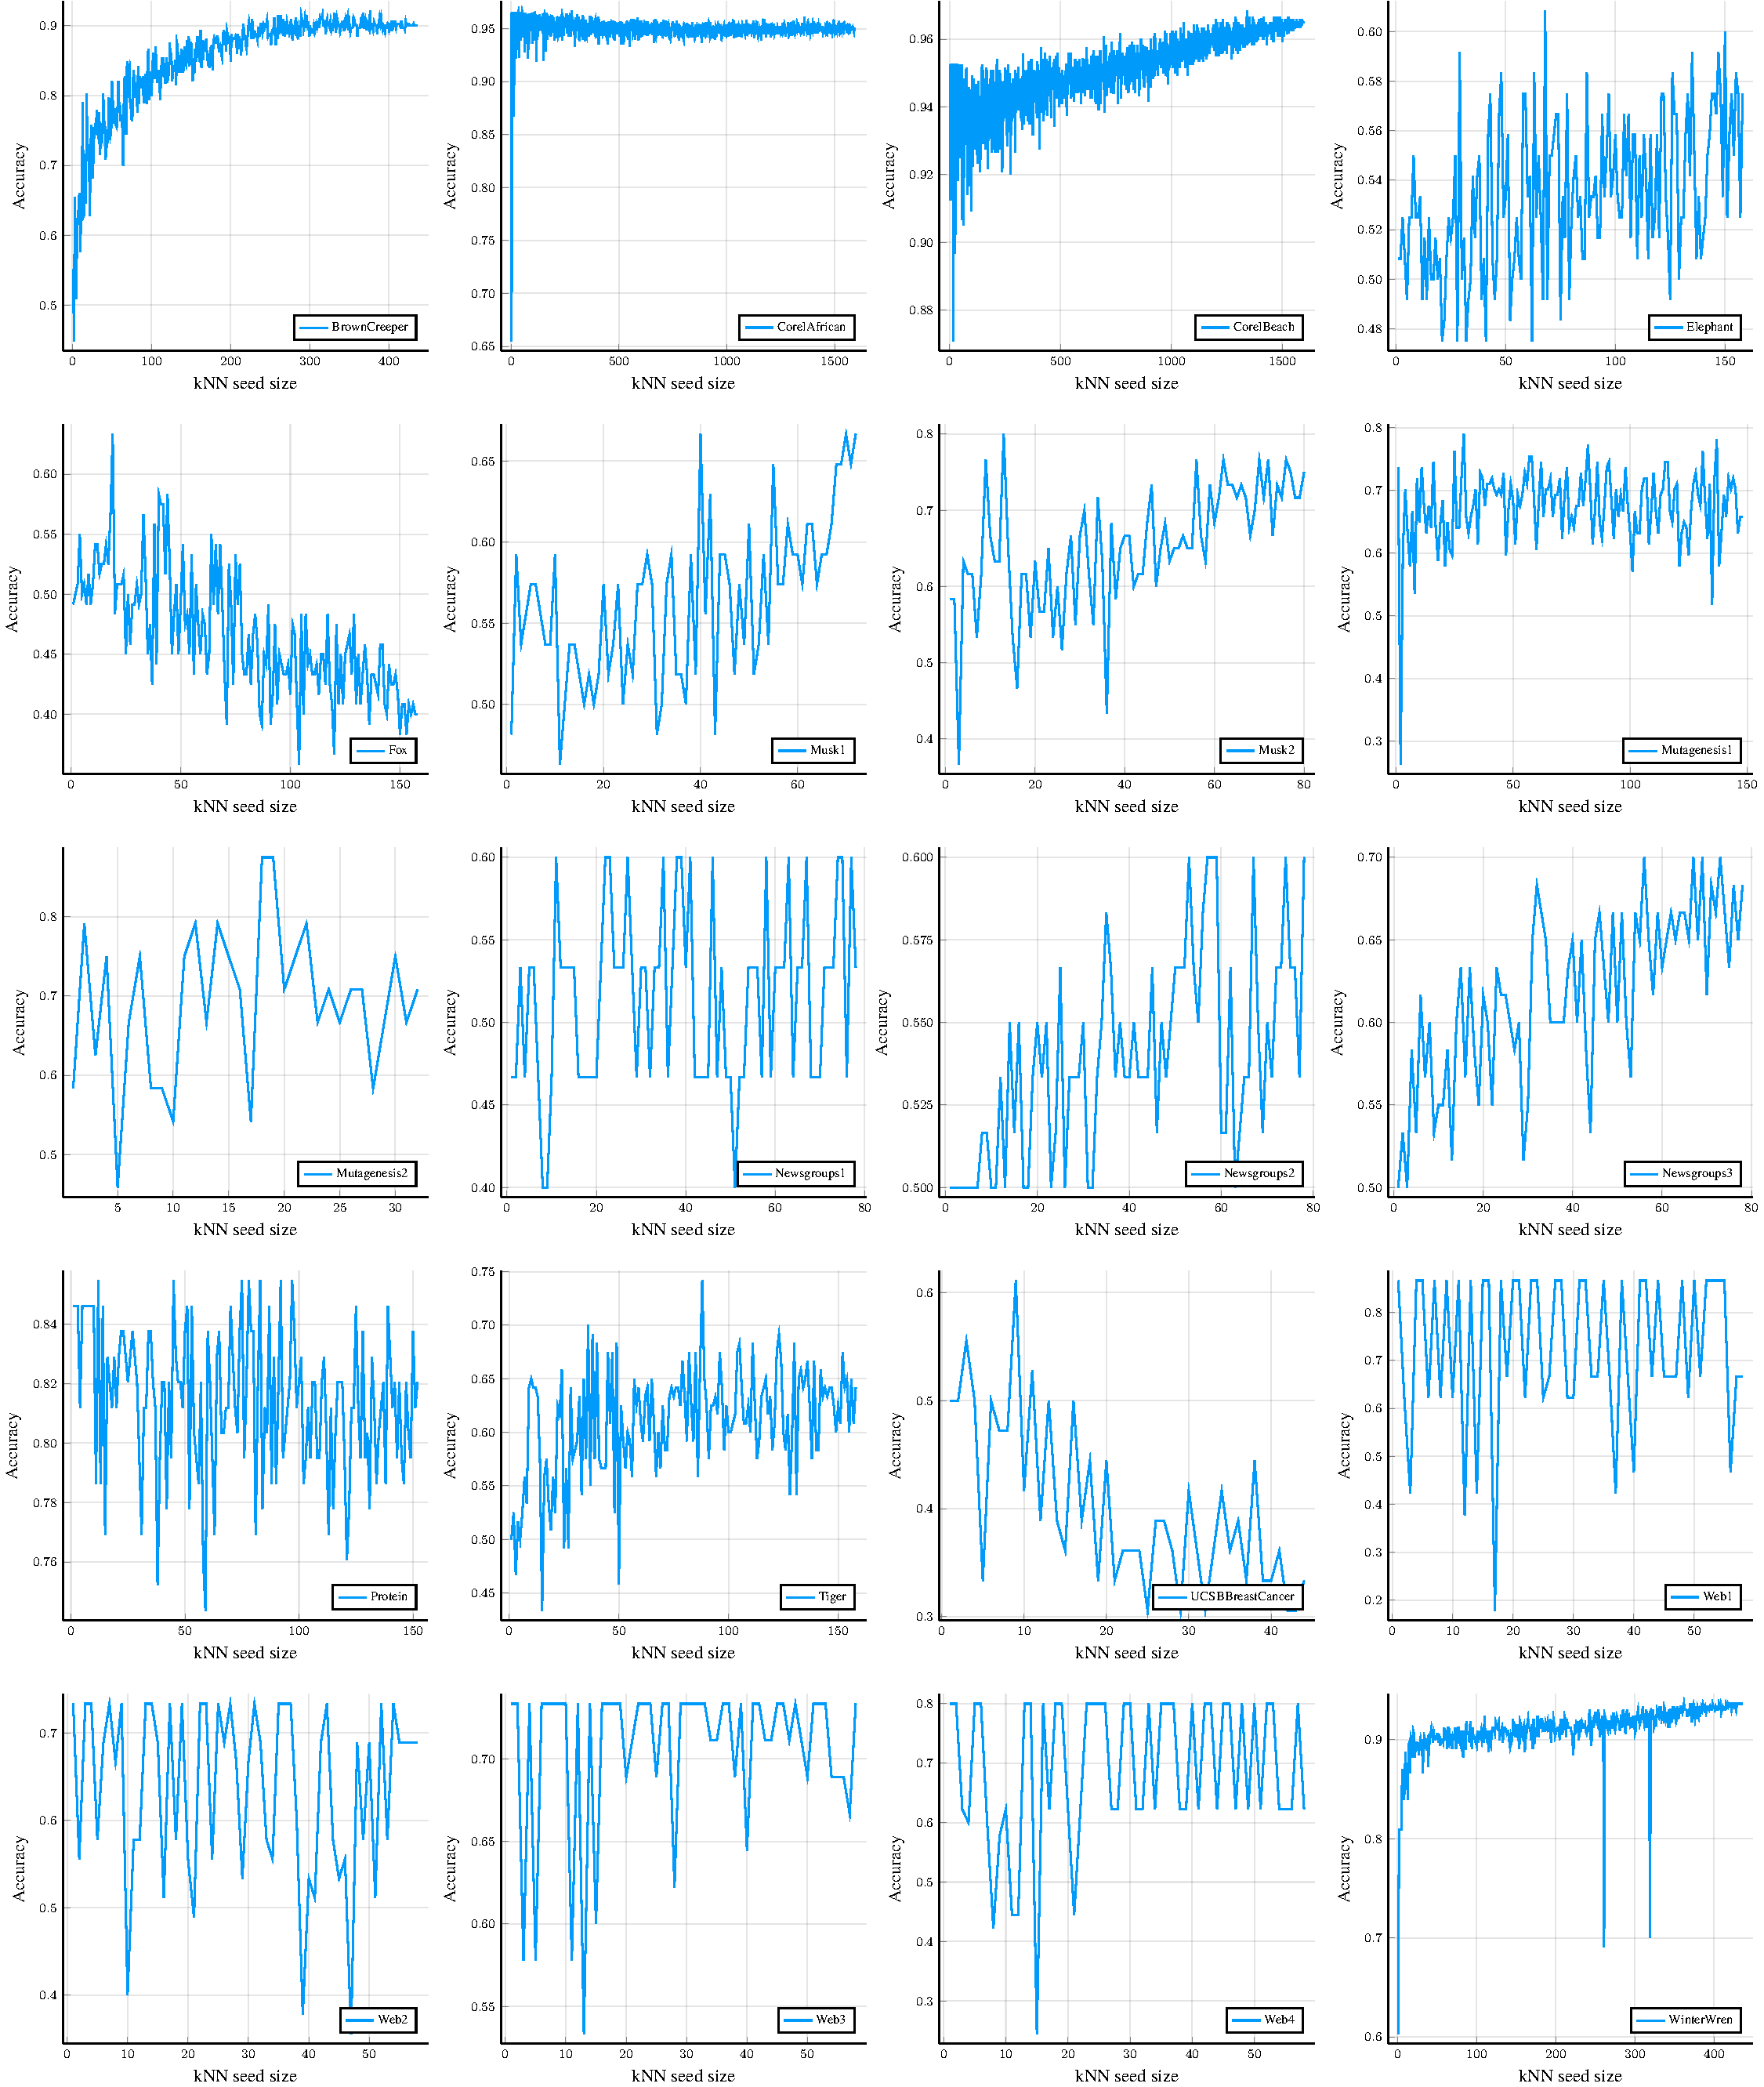
\includegraphics[width=\textwidth]{images/CPC-toy/kNN/CPC-toy-kNN.pdf}
  \caption{The accuracy of a kNN classifier built on the final embedding for \( L_\mathrm{CPC} \) as a function of the number of samples used to seed it. Average of three runs.}\label{fig:CPC-toy-kNN}
\end{figure}

\begin{figure}
  \centering
  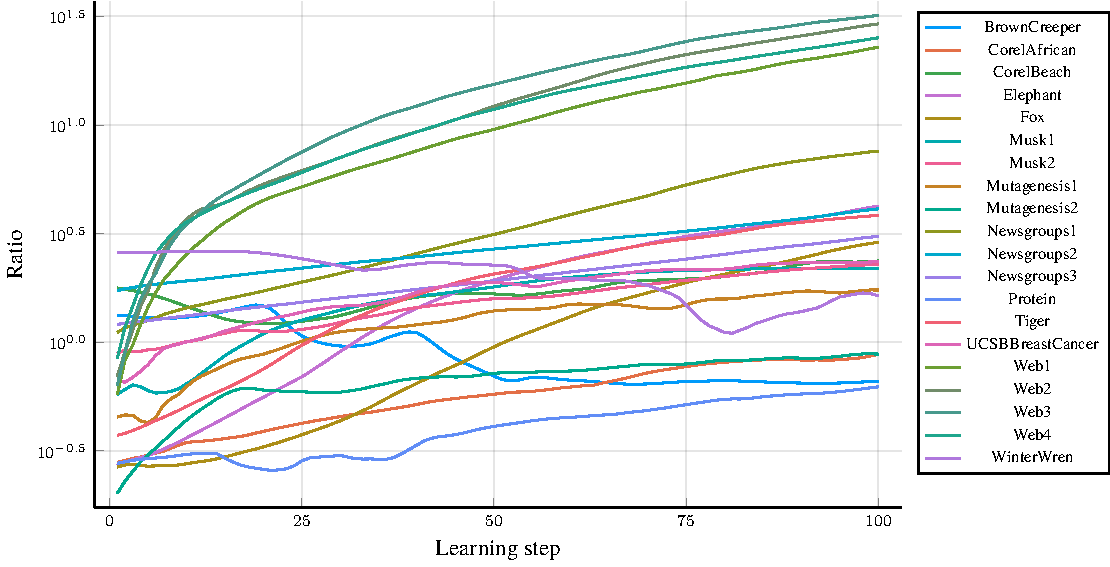
\includegraphics[width=\textwidth]{images/triplet-toy/ratio/triplet-toy-ratio.pdf}
  \caption{The value of \( \mathrm{silhouette} \left( \cdot \right) \) for triplet loss over the learning period. Note the logarithmic scale on the \( y \) axis.}\label{fig:triplet-toy-ratio}
\end{figure}

\begin{figure}
  \centering
  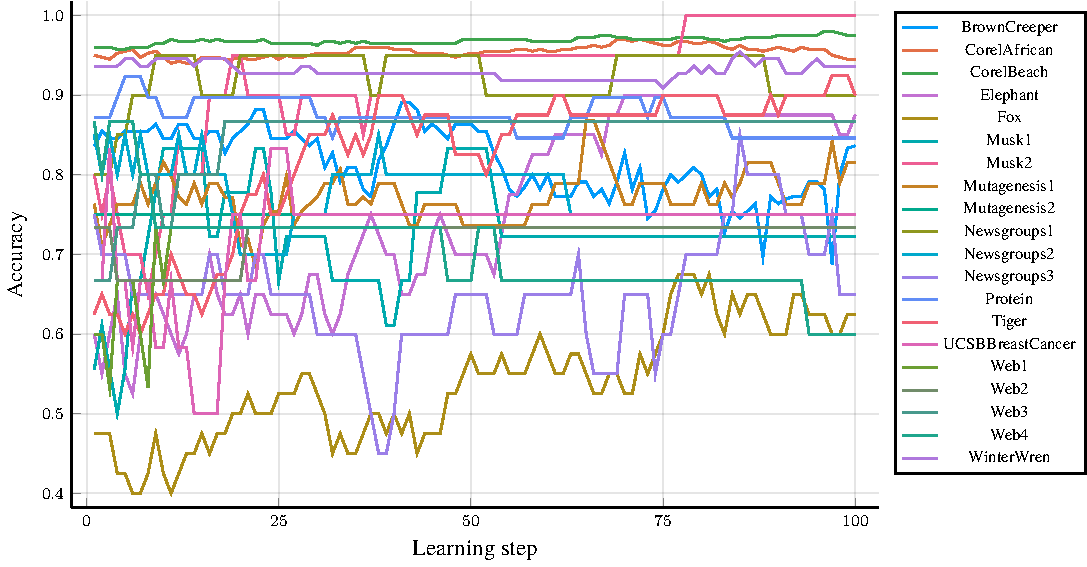
\includegraphics[width=\textwidth]{images/triplet-toy/accuracy/triplet-toy-accuracy.pdf}
  \caption{The accuracy of a kNN classifier built on the embedding for triplet loss over the learning period.}\label{fig:triplet-toy-accuracy}
\end{figure}

\begin{figure}
  \centering
  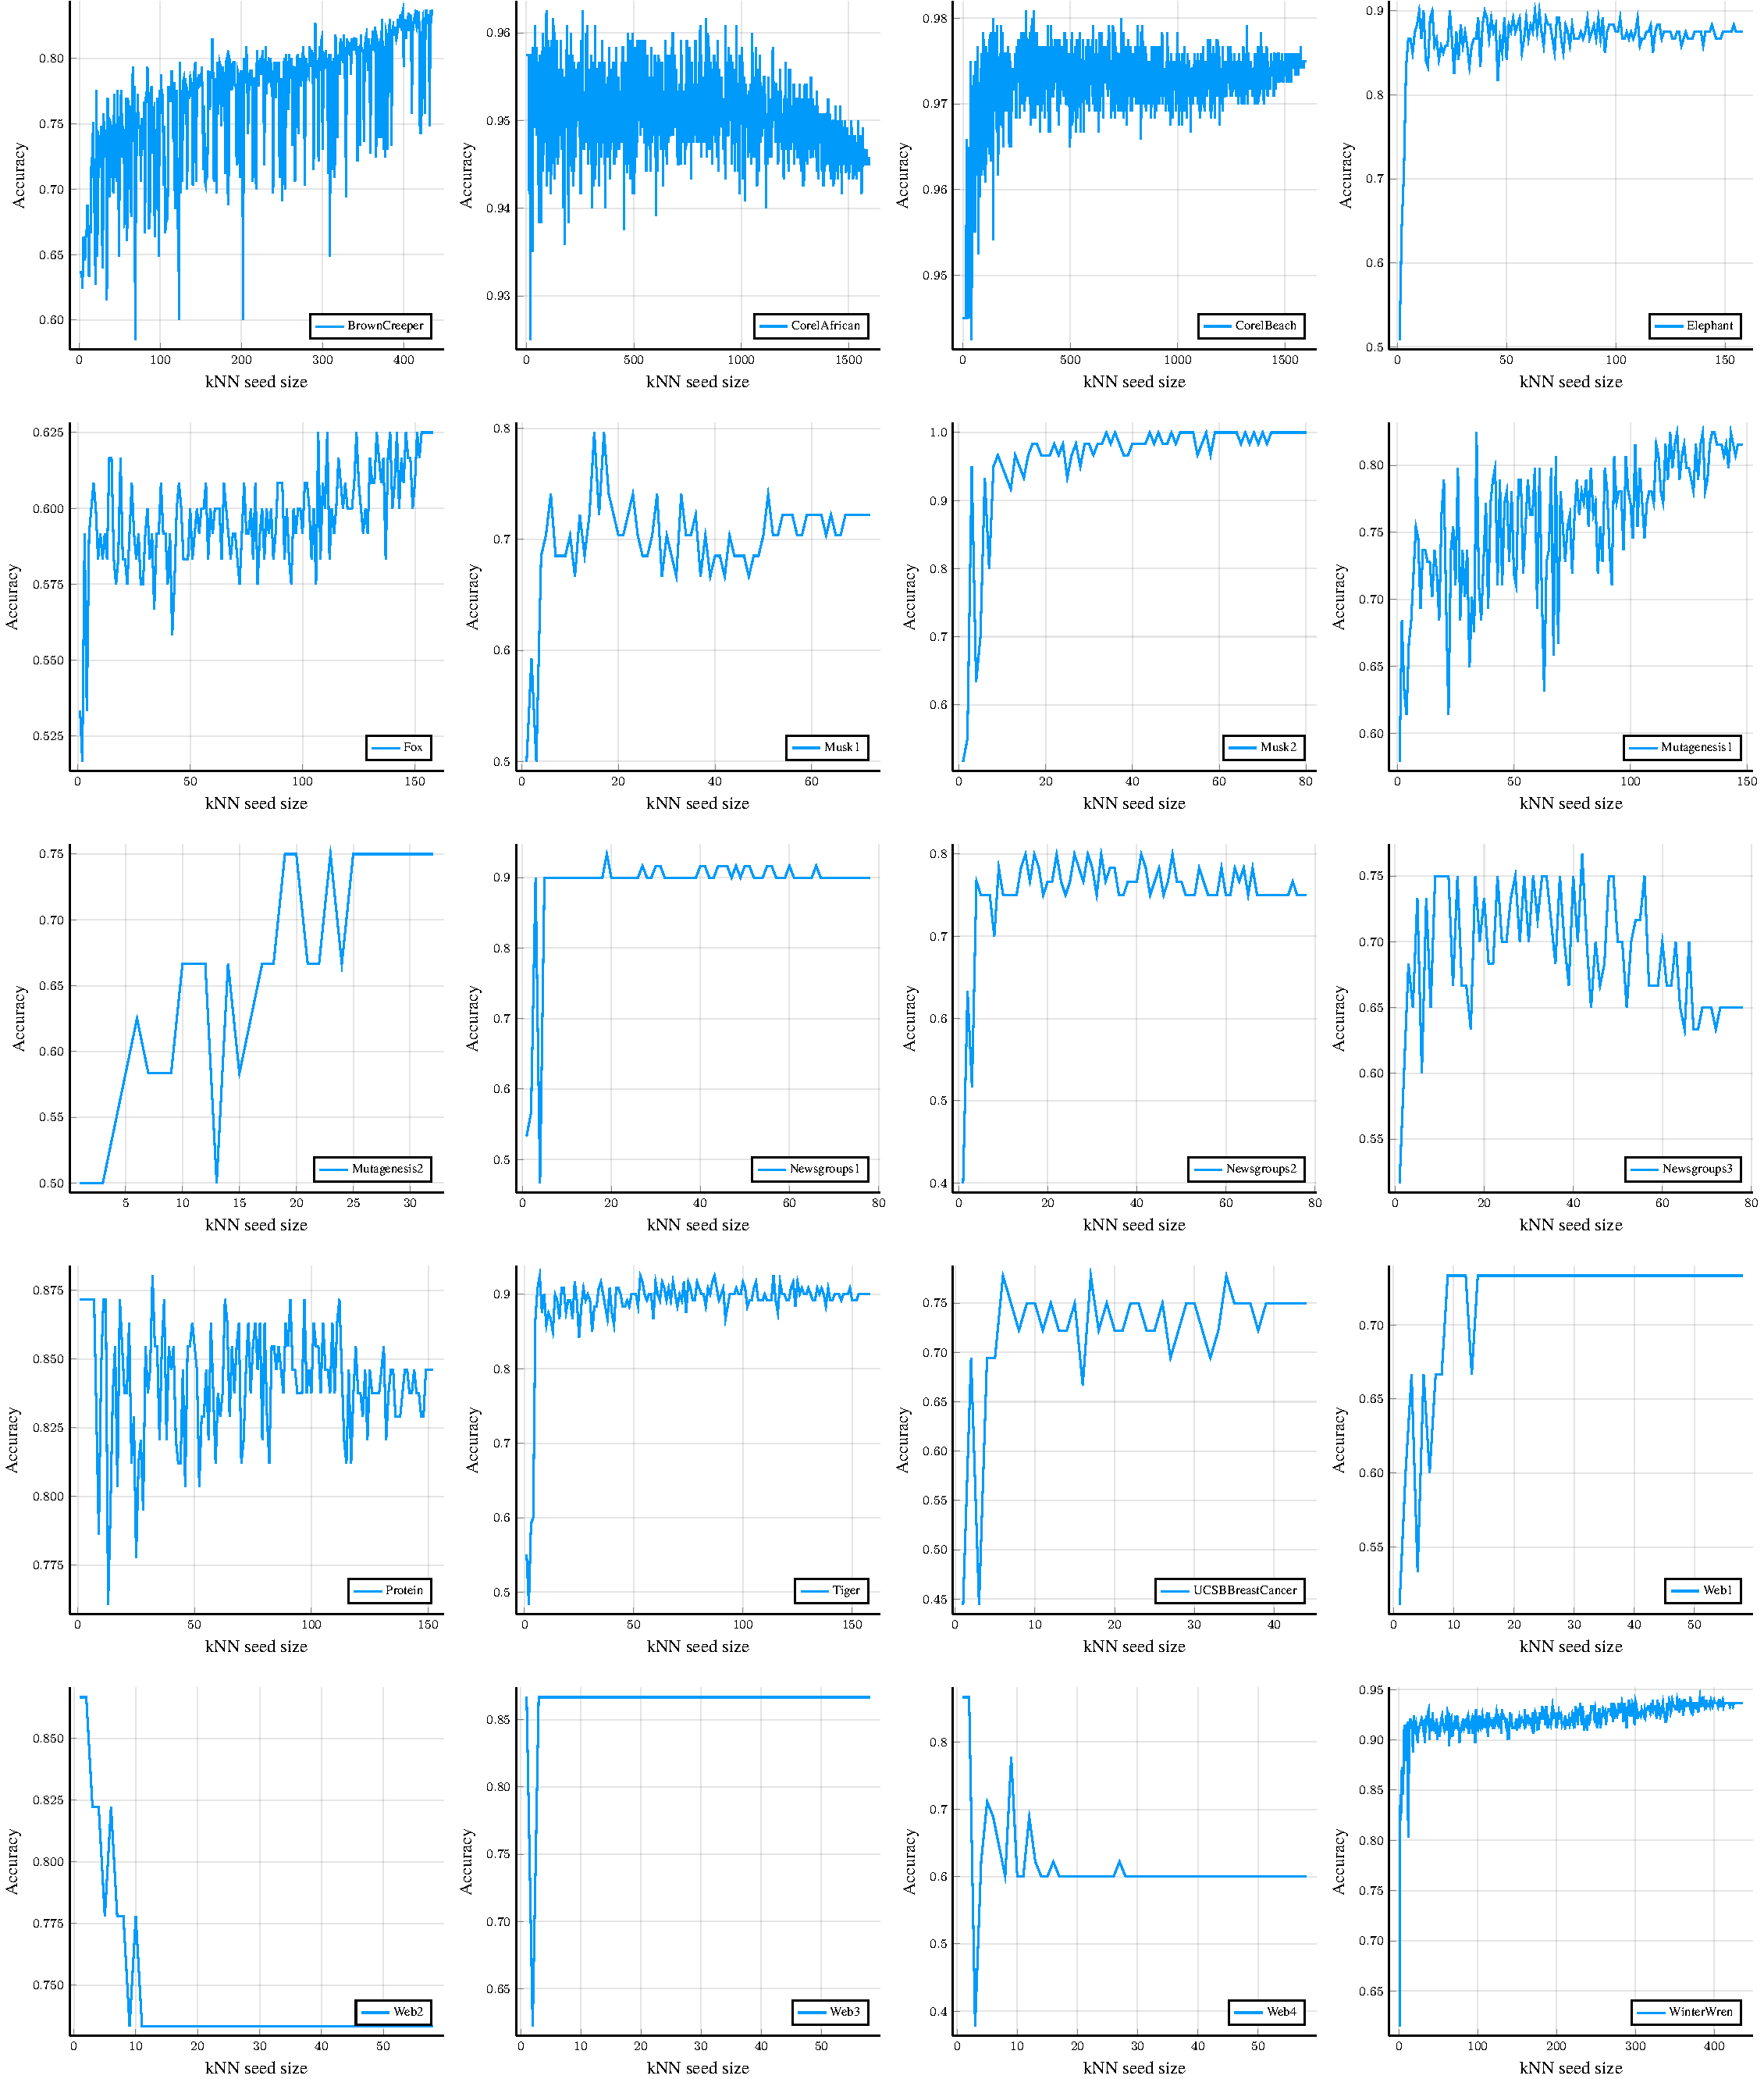
\includegraphics[width=\textwidth]{images/triplet-toy/kNN/triplet-toy-kNN.pdf}
  \caption{The accuracy of a kNN classifier built on the final embedding for triplet loss as a function of the number of samples used to seed it. Average of three runs.}\label{fig:triplet-toy-kNN}
\end{figure}

\begin{figure}
  \centering
  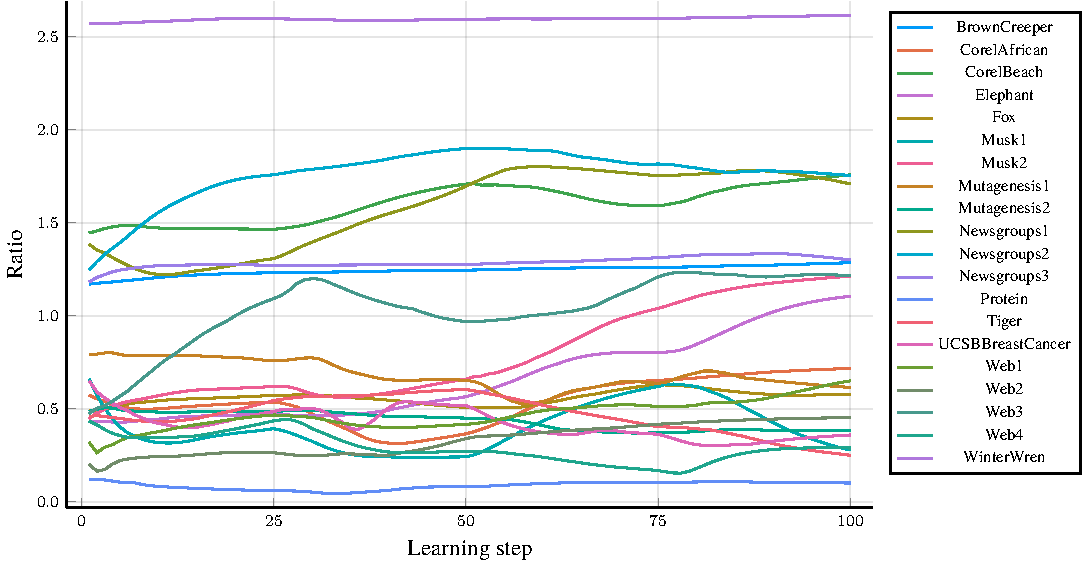
\includegraphics[width=\textwidth]{images/magnet-toy/ratio/magnet-toy-ratio.pdf}
  \caption{The value of \( \mathrm{silhouette} \left( \cdot \right) \) for magnet loss over the learning period. Note the logarithmic scale on the \( y \) axis.}\label{fig:magnet-toy-ratio}
\end{figure}

\begin{figure}
  \centering
  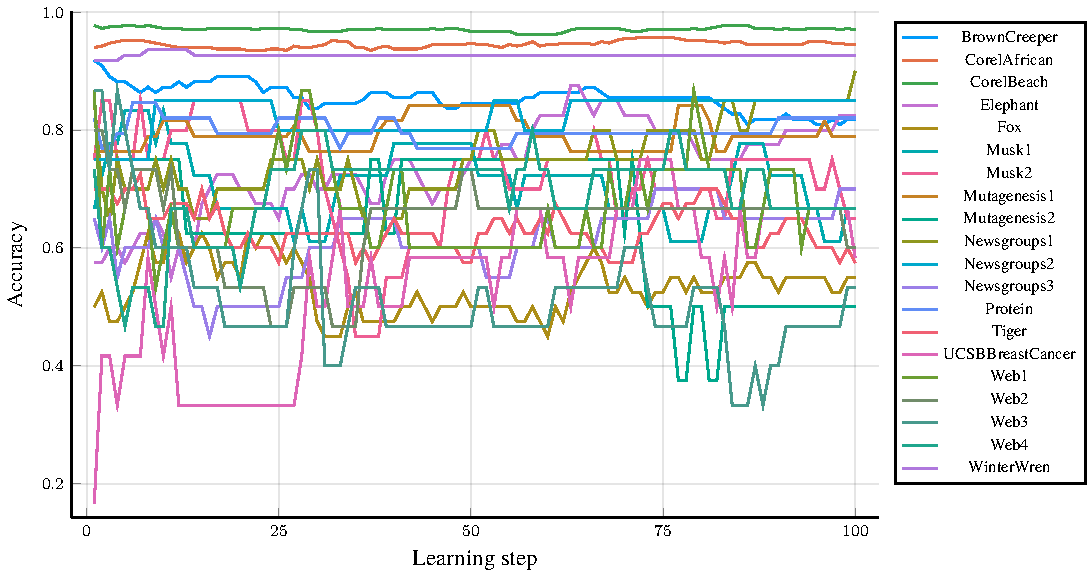
\includegraphics[width=\textwidth]{images/magnet-toy/accuracy/magnet-toy-accuracy.pdf}
  \caption{The accuracy of a kNN classifier built on the embedding for magnet loss over the learning period.}\label{fig:magnet-toy-accuracy}
\end{figure}

\begin{figure}
  \centering
  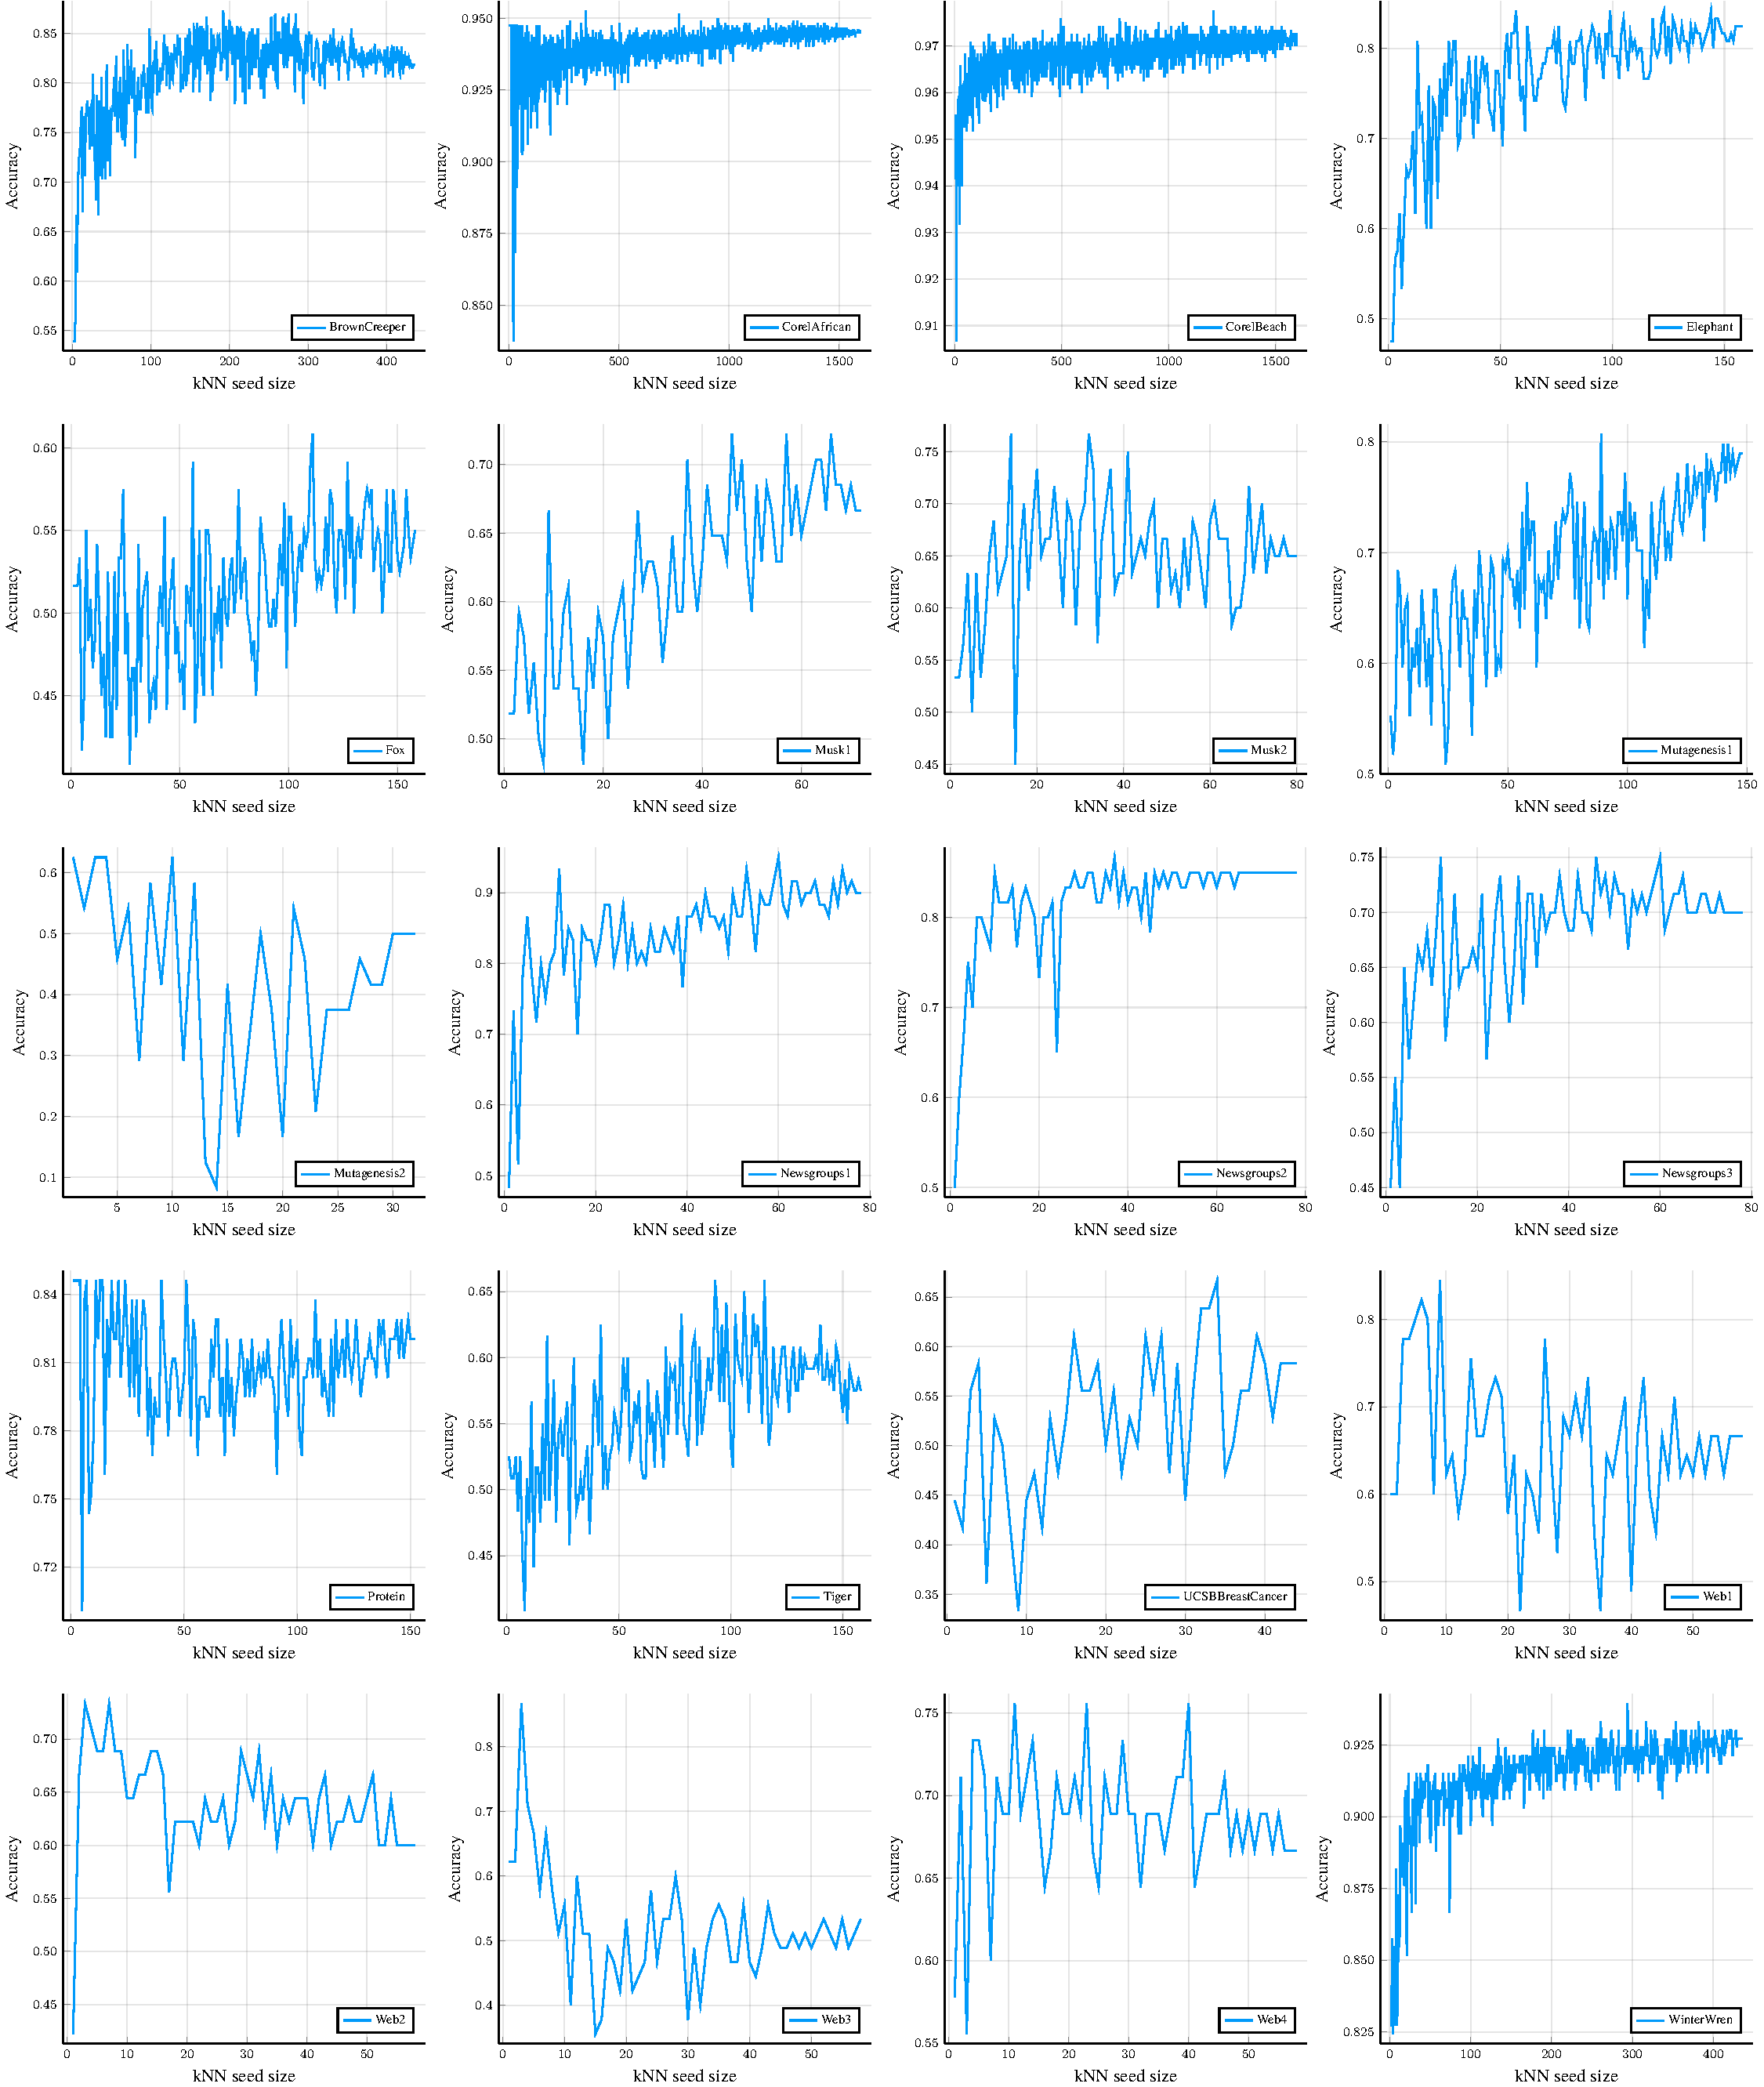
\includegraphics[width=\textwidth]{images/magnet-toy/kNN/magnet-toy-kNN.pdf}
  \caption{The accuracy of a kNN classifier built on the final embedding for magnet loss as a function of the number of samples used to seed it. Average of three runs.}\label{fig:magnet-toy-kNN}
\end{figure}

\begin{figure}
  \centering
  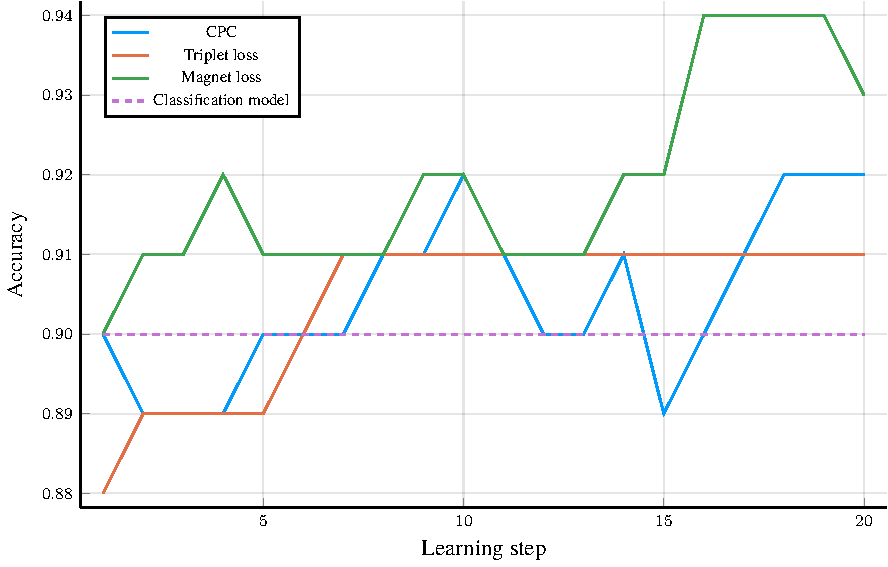
\includegraphics[width=0.75\textwidth]{images/cisco/accuracy/cisco-accuracy.pdf}
  \caption{The accuracy of a kNN classifier built on the final embedding over the learning period. Average of three runs on the corporate dataset.}\label{fig:cisco-accuracy}
\end{figure}

\begin{figure}
  \centering
  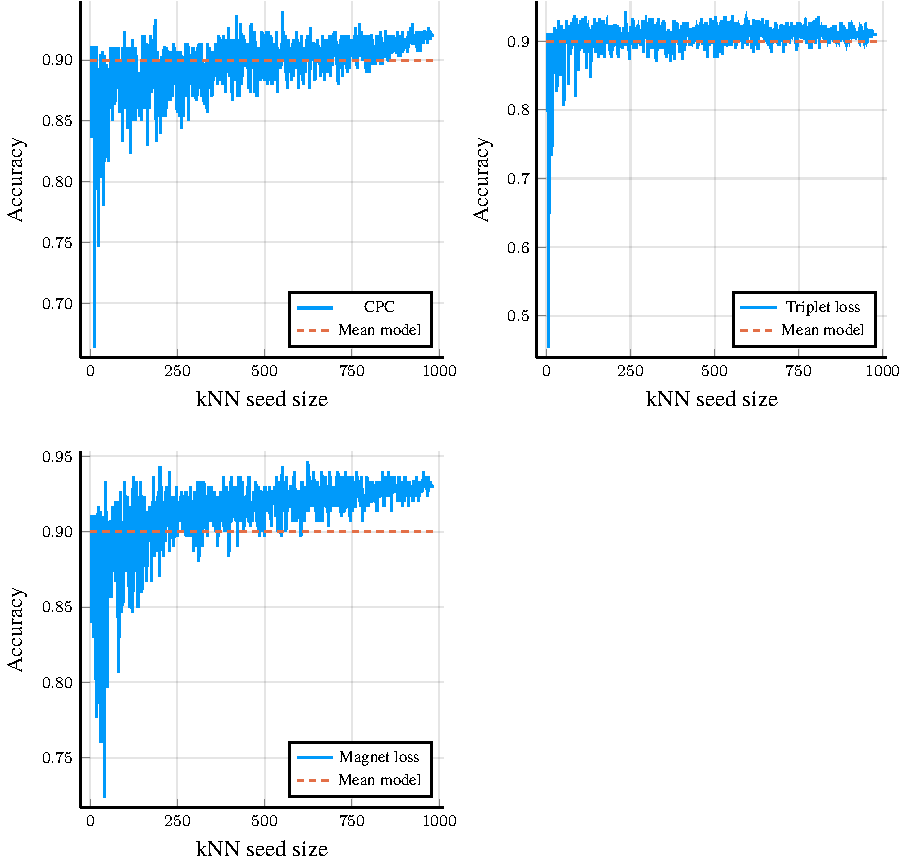
\includegraphics[width=0.75\textwidth]{images/cisco/kNN/cisco-kNN.pdf}
  \caption{The accuracy of a kNN classifier built on the final embedding as a function of the number of samples used to seed it. Average of three runs on the corporate dataset.}\label{fig:cisco-kNN}
\end{figure}

\begin{figure}
  \centering
  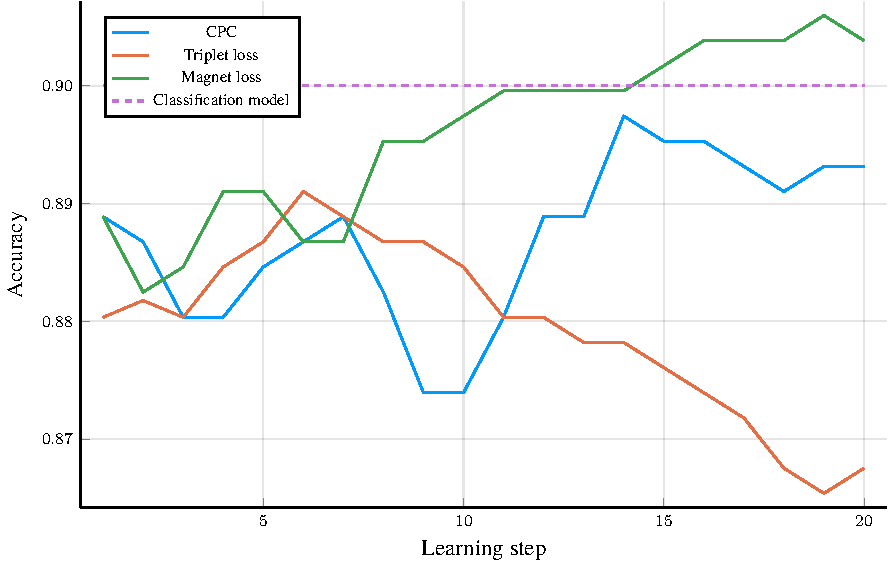
\includegraphics[width=0.75\textwidth]{images/cisco-multiclass/accuracy/cisco-multiclass-accuracy.pdf}
  \caption{The accuracy of a kNN classifier built on the final embedding over the learning period. Average of three runs on the corporate dataset with 20 classes.}\label{fig:cisco-multiclass-accuracy}
\end{figure}

\begin{figure}
  \centering
  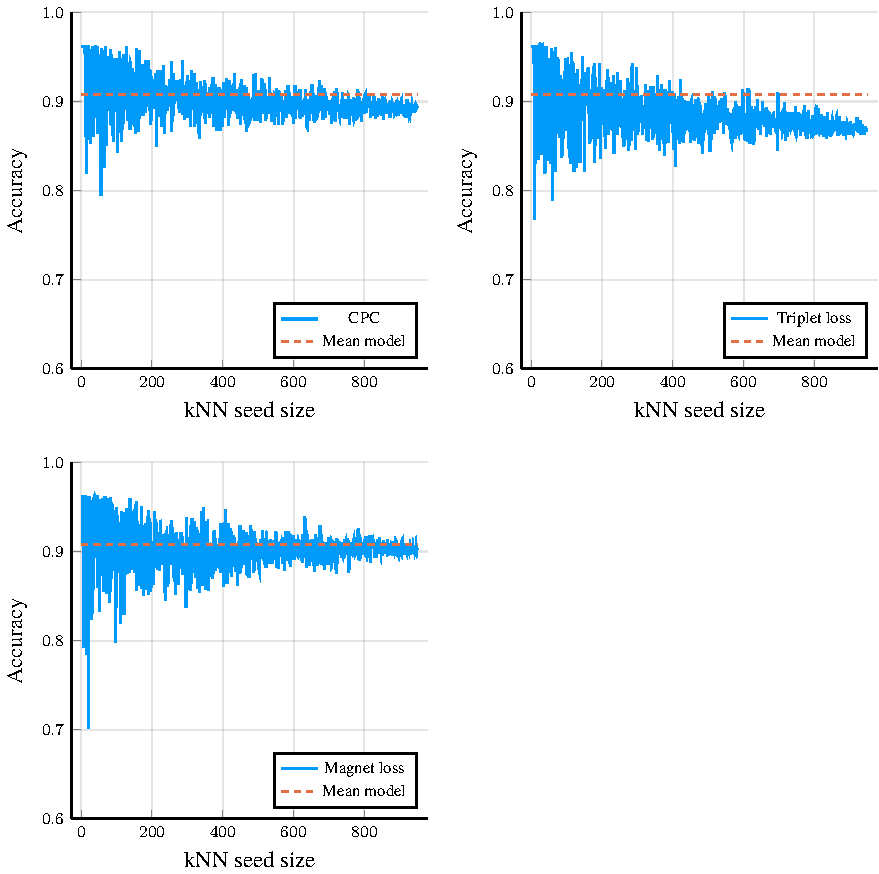
\includegraphics[width=0.75\textwidth]{images/cisco-multiclass/kNN/cisco-multiclass-kNN.pdf}
  \caption{The accuracy of a kNN classifier built on the final embedding as a function of the number of samples used to seed it. Average of three runs on the corporate dataset with 20 classes.}\label{fig:cisco-multiclass-kNN}
\end{figure}
